\documentclass[presentation,xcolor={usenames,dvipsnames},10pt]{beamer}

% figures
\newcommand{\home}{.}
\newcommand{\figures}{\home/figures}
\input formatting.tex
\input defs.tex
\usepackage{hyperref}
\hypersetup{colorlinks=true}

\newcommand{\norm}[1]{\left\lVert{#1}\right\rVert}
\newcommand{\Diag}{\text{diag}}
%\newcommand{\minimize}[1]{\underset{{#1}}{\text{minimize}}}
\newcommand{\tTheta}{\widetilde{\Theta}}
\newcommand{\numinputs}{d}
\newcommand{\numoutputs}{k}
\newcommand{\numhiddens}{H}
\newcommand{\vu}{\boldsymbol{u}}
\newcommand{\vv}{\boldsymbol{v}}
\newcommand{\vx}{\boldsymbol{x}}
\newcommand{\vy}{\boldsymbol{y}}
\newcommand{\mU}{\boldsymbol{U}}
\newcommand{\mV}{\boldsymbol{V}}
\newcommand{\mW}{\boldsymbol{W}}
\newcommand{\rect}{\text{rect}}
\newcommand{\gpath}{\text{path}}
\newcommand{\layer}{\text{layer}}
\newcommand{\DAG}{\text{DAG}}
\newcommand{\dout}{d_\text{out}}
\newcommand{\din}{d_\text{in}}
\newcommand{\IN}{\text{in}}
\newcommand{\OUT}{\text{out}}
\newtheorem{claim}{Claim}
\newenvironment{sketch}{\paragraph{Proof sketch}\mbox{}}{\hfill\BlackBox}
\newcommand{\vin}{v_{in}}
\newcommand{\vout}{v_{out}}
\newcommand{\relu}{\sigma_{\textsc{relu}}}
\newcommand{\gnorm}[1]{\norm{#1}}
\newcommand{\mugeom}{\mu^{\textit{geo}}}
\newcommand{\pathr}{\phi}
\newcommand{\convexnn}{\nu}
\newcommand{\RSGD}{Path-SGD }



% \mode<handout>
% %\mode<presentation>
{
\usetheme{default}
}
\setbeamertemplate{footline}[frame number]

\bibliographystyle{alpha}

\title{Path-SGD: Path-Normalized Optimization in Deep Neural Networks}

\date{\textcolor{blue}{\today}}
\author{Ramchandran Muthukumar}

\begin{document}

\begin{frame}
\titlepage
\end{frame}

\section{Geometry}

\begin{frame}{Motivation - Link Between Geometry and Optimization Algorithms}
\bit 
\item Geometry = measure of distance, norm or divergence. 

\item Some hoices are $\ell_1$ and $\ell_2$ norms. 

\item Optimization algorithms are tied to geometry inherently. 

\item Gradient descent = steepest descent w.r.t. $\ell_2$ norm. 

\item Coordinate descent = steepest descent w.r.t.  $\ell_1$ norm. 

\eit 
\end{frame}

\begin{frame}{Impact of geometry on learning}
\bit 

\item The choice of geometry $\Rightarrow$ a choice of regularization on weights. 

\item Ideal properties of a geometry -
\begin{enumerate}
	\item faster optimization
	\item better implicit regularization 
\end{enumerate}
\item Is $\ell_2$ geometry the best choice for learning deep neural networks?
\eit 
\end{frame}

\begin{frame}{Notations}

\begin{definition}[RELU Feed-forward Neural Network]
A feed-forward neural network computes a function $f:\mathbb{R}^D \rightarrow \mathbb{R}^C$.

It is defined by a directed acyclic graph $G(V,E)$ with 
\begin{enumerate} 
	\item $D$ input nodes
	$\vin[1],\dots,\vin[D]\in V$
	\item $C$ output nodes $\vout[1],\dots,
	\vout[C]\in V$.
\end{enumerate}

For two vertices $u_1,u_2 \in V$, the weight on the corresponding edge $u_1\rightarrow u_2$ is denoted as $w_{(u_1\rightarrow u_2)} \in \mathbb{R}$. 

The network is parameterized by the collection of edge weights $\mathbf{w}$.

The activation function
$\relu(x) = \max\{0,x\}$ acts on the internal nodes (hidden
units).

We denote the function computed by this network as
$f_{G,\mathbf{w},\relu}$. 
\end{definition}

\end{frame}


\begin{frame}{RELU Networks are Rescaling Invariant}

\begin{figure}
	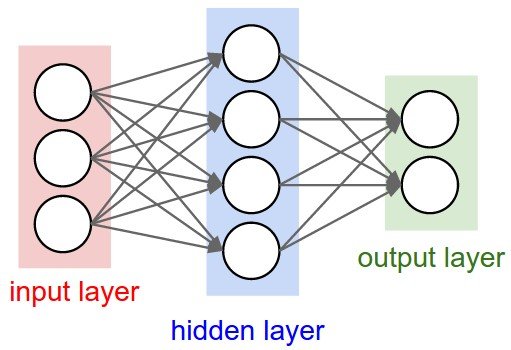
\includegraphics[scale=0.2]{neural_net.jpeg}
\end{figure}


\bit 
\item Consider any hidden unit $v$.

\item Scale down the incoming edges to $v$ by a factor $c$

\item Scale up the outgoing edges from $v$ by the same factor $c$.

\item The resulting network still computes the same function. 

\item Therefore RELU Networks are invariant to such a rescaling. 
\eit 
\end{frame} 

\begin{frame}{Mathematical description of rescaling}
\begin{lemma}
RELU activation is non-negative homogeneous. For any scalar $c \geq 0$ and any $x \in \mathbb{R}$, $\relu(cx) = c\relu(x)$. 
\end{lemma}

\begin{definition}[Rescaling Function]
For any node $v \in V$, a scaling factor $c > 0$ and the weights of the network $\mathbf{w}$ , We define the {\em rescaling function} $\rho_{c,v}(\cdot) : w \mapsto \tilde{w}$ such that for all edges $(u_1\rightarrow u_2)\in E$,
\begin{equation}
\tilde{w}_{(u_1\rightarrow u_2)}=
\begin{cases}
cw_{(u_1\rightarrow u_2)}& u_2=v,\\
\frac{1}{c}w_{(u_1\rightarrow u_2)}& u_1=v,\\
w_{(u_1\rightarrow u_2)}& \text{otherwise.}\\
\end{cases}
\end{equation}
\end{definition}

A network rescaled with $\rho_{c,v}(\cdot)$ computes the same function, i.e. 
$$f_{G,\mathbf{w},\relu} = f_{G,\rho_{c,v}(\mathbf{w}),\relu}$$.

\end{frame}

\begin{frame}{Rescaling Invariance}
\begin{definition}[Rescaling Equivalent Networks]
Two RELU feedforward neural networks defined on the graph $G(V,E)$ with weights $w$ and $\tilde{w}$ are {\em rescaling equivalent} if and only if one of them can be transformed to another by applying a sequence of rescaling functions $\rho_{c,v}$.
	
We denote this property by $w\sim \tilde{w}$
\end{definition}
\end{frame}

\begin{frame}{Rescaling Invariance}
\begin{definition}[Rescaling Invariant Optimization Method]
An optimization method is {\em rescaling invariant} if its updates on rescaling equivalent networks are rescaling equivalent.

Let the initial weight matrices from rescaling equivalent  networks are $\tilde{w}^{(0)}\sim w^{(0)}$. 

For all iterations $t$ under the optimization method, the weight matrices remain rescaling equivalent and we have $\tilde{w}^{(t)} \sim
w^{(t)}$.	
\end{definition}
\end{frame}

\begin{frame}{Rescaling and Unbalanced Networks}
\begin{definition}[Balanced Networks]
We say that a network is {\em balanced} if the norm of
incoming weights to different units are roughly the same or within a
small range. 
\end{definition}

Balanced networks can be rescaled to equivalent unbalanced networks. 

Gradient descent and SGD perform very poorly on ``unbalanced''
networks.  

\begin{figure}
	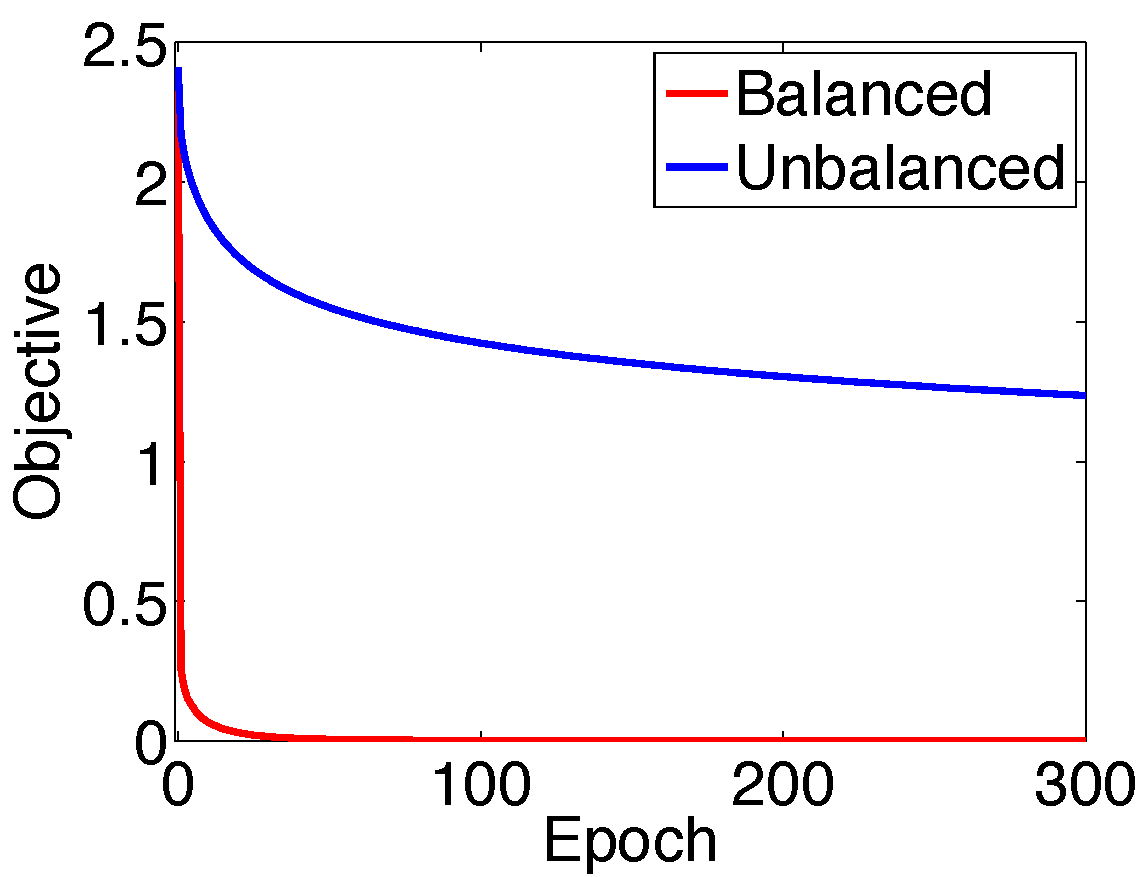
\includegraphics[scale=0.2]{mnist-compare.pdf}
	\caption{Comparison of SGD on equivalent balanced and unbalanced networks for training on MNIST}
\end{figure}

\end{frame}

\begin{frame}{Issues with Unbalanced Networks}

\bit
\item Gradient descent is \emph{not} rescaling invariant. 
\item Scaling down the weights of an edge will scale up the gradient. 
\item Larger weights remain almost unchanged 
\item Smaller weights blow up

\begin{figure}
	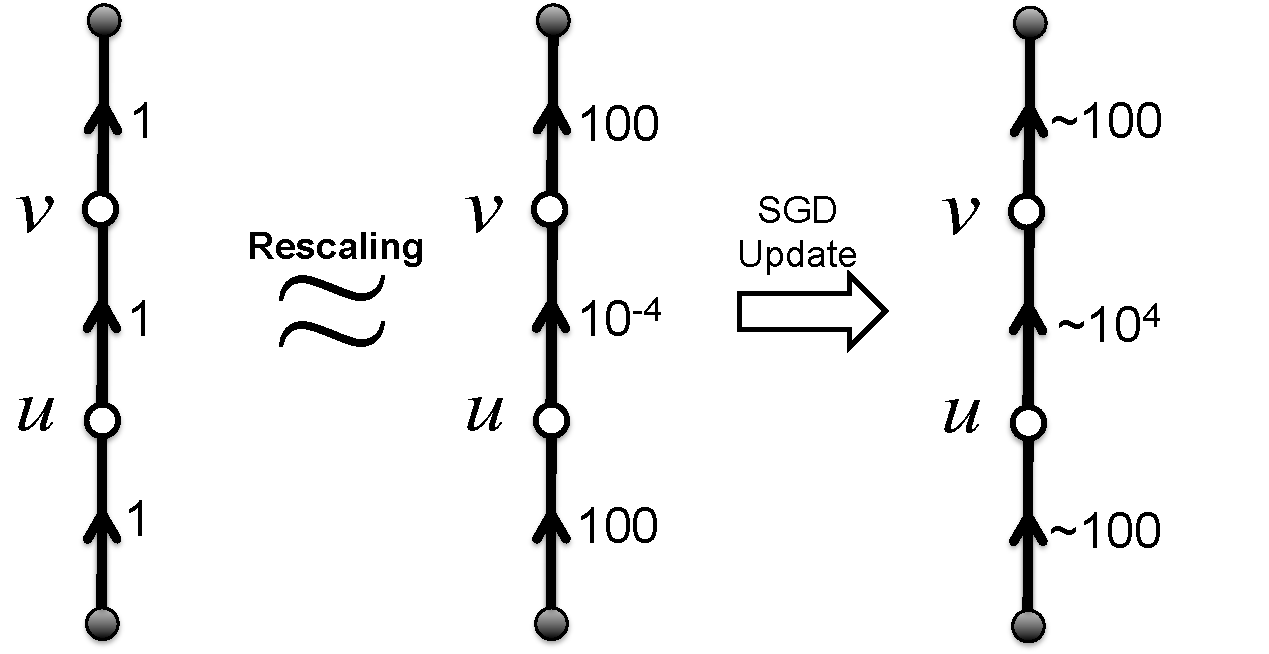
\includegraphics[scale=0.3]{pic3.pdf}
	%\caption{}
\end{figure}

\item Can you think of a way to fix this?

\eit
\end{frame}


\begin{frame}{Possible Fix?}
\bit 
\item We can rescale the weights after each update to a more balanced network.
\eit 
\end{frame} 

\begin{frame}{Additional Issues with Unbalanced Network}
\bit 
\item Very different relative changes in weights compared to a balanced network. 

\begin{figure}
	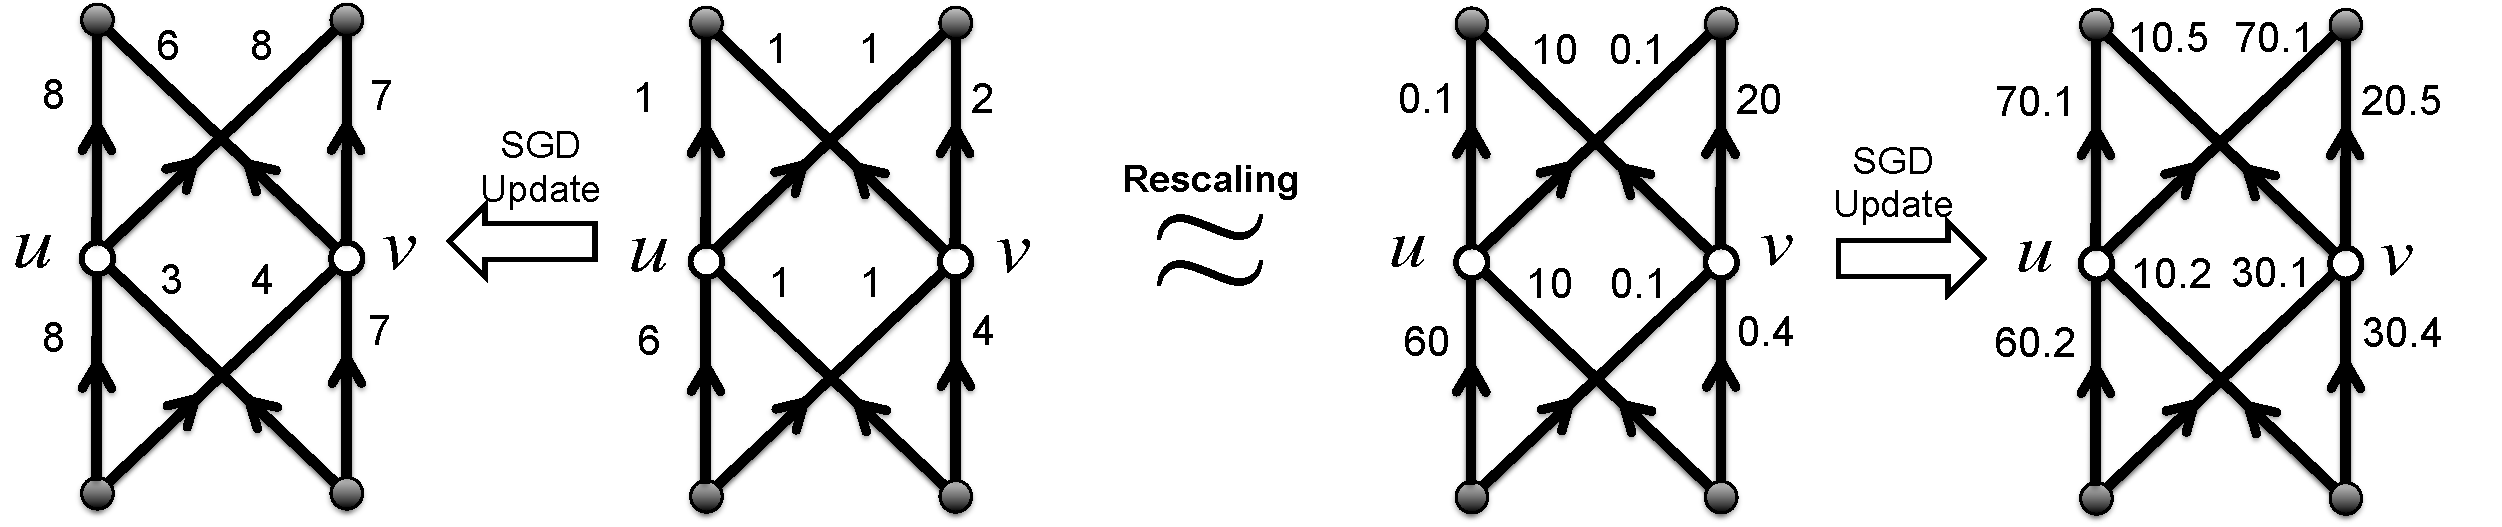
\includegraphics[scale=0.24]{pic4.pdf}
\end{figure}
\item After just a single update two rescaling equivalent networks could end up computing very different functions
\eit
\end{frame}

\begin{frame}{Rescaling Invariant}

\bit 
\item Predictions (or function computed) by RELU Feed-forward neural networks are rescaling invariant.
\item We want a geometry and a corresponding optimization method that is also rescaling invariant 

\item This paper considers a rescaling invariant geometry inspired by max-norm regularization.

\eit 

\end{frame}


\begin{frame}{Scale measures for deep networks}
\begin{definition}[Group-Norm Regularizer]
The generic group-norm regularizer
parametrized by $1\leq p,q \leq\infty$ is defined as
\begin{equation*}
\label{eq:mu}
\mu_{p,q}(w) = \left(\sum_{v \in V}\left(\sum_{(u\rightarrow v) \in E} \left\lvert w_{(u\rightarrow v)}\right\rvert ^p\right)^{q/p}\right)^{1/q}.
\end{equation*} 
\end{definition}

\bit
\item When $p=q=1$ this is $\ell_1$ regularization. 
\item When $p=q=2$ this is weight decay (most commonly used). 
\eit 

\begin{definition}[Max-norm regularizer]
The max-norm regularizer is defined as 
\begin{equation*}
\label{eq:mu}
\mu_{p,\infty}(w) =\sup_{v \in V}\left(\sum_{(u\rightarrow v) \in E} \left\lvert w_{(u\rightarrow v)}\right\rvert ^p\right)^{1/p}
\end{equation*}

This is equivalent to setting $q=\infty$ in the per-unit regularizer. 
\end{definition}
\end{frame}

\begin{frame}{Usage of Max-norm regularizer}

\bit
\item Max-norm regularization is
extreme because the value of regularizer corresponds to
the highest value among all nodes.

\item But it has empirically been shown to be effective for RELU networks. 

\item This could be because of RELU networks can be rebalanced such that all hidden units have the similar norm. 

\item The max-norm regularizer $\mu_{p,\infty}$ is also \textbf{not} rescaling invariant.

\item We want a rescaling-invariant regularizer. 

\item We can instead look for the minimum value of the max-norm regularizer among all rescaling equivalent networks. 
\eit

\end{frame}

\begin{frame}{Paths in Feed-forward neural network}

\begin{definition}[Path vector]
Consider a RELU feed-forward
network parameterized by the graph $G(V,E)$ and edge weights $\mathbf{w}$.

Let $P_{i,j} = \{e_1,e_2,\ldots,e_d\}$ be a path from the $i$-th input unit $v_{in}[i]$ to the $j$-th output unit $v_{out}[j]$. Let $|P|$ be the number of such unique paths. 

The {\em path vector} $\pi(\textbf{w}) \in \mathbb{R}^{|P|}$ is defined as the vector where each co-ordinate is the product of all weights along a path. 
 
$$\displaystyle \pi_{P_{i,j}}(\mathbf{w}) = \prod_{k=1}^d \mathbf{w}_{e_k}$$
\end{definition}
\end{frame}

\begin{frame}{$\ell_p$-path regularizer}
\begin{definition}[$\ell_p$-path regularizer]
The $\ell_p$-path regularizer $\phi_p(\mathbf{w})$ is defined as the $\ell_p$ norm of
$\pi(\textbf{w})$:
\begin{equation}\label{eq:defphi}
\phi_p(\textbf{w}) = \norm{\pi(\textbf{w})}_p = 
\left(\sum_{\vin[i] \overset{e_1}\rightarrow v_1\overset{e_2}\rightarrow v_2\dots\overset{e_d}{\rightarrow}\vout[j]} \left|\prod_{k=1}^d \textbf{w}_{e_k}\right|^p\right)^{1/p}
\end{equation}

\end{definition}

\bit 
\item What would be the complexity of computing $\phi_p(\mathbf{w})$ ? 
\eit
\end{frame}

\begin{frame}{Computation of $\ell_p$-path regularizer}
\bit 
\item The $\ell_p$-path regularizer can be computed
efficiently in a \emph{single forward step} by the following recursive definition 

\begin{align*}
\phi_{p,v}(\mathbf{w}) &= \sum_{(u\rightarrow v)\in E} \phi_{p,u}(\mathbf{w}) \cdot (\mathbf{w}_{u \rightarrow v})^p\ \\
\phi_{p}(\mathbf{w}) & = \sum_{u\in V_{out}} \phi_{p,u}(\mathbf{w})
\end{align*}
\eit 

\end{frame} 

\begin{frame}{Link between $\ell_p$-path regularizer and max-norm regularizer}
\bit 

\begin{lemma}
	The $\ell_p$-path regularizer and per-unit regularizer satisfy the following relation :
	$$\displaystyle \phi_p(w) = \min_{\tilde{w} \sim w} \bigg(\mu_{p,\infty}(\tilde{w})\bigg)^d$$
where $d$ is the depth of the neural network. 
\end{lemma}

\item Hence the $\ell_p$ path-regularizer $\phi_p$ is invariant to rescaling. 

 For any $\tilde{w} \sim w$, $\phi_p(\tilde{w})=\phi_p(w)$
\eit 
\end{frame}

\section{Path-SGD: Approximate Path-Regularized Steepest Descent}
\begin{frame}{Steepest Descent w.r.t. $\ell_p$-path regularizer}
\bit
\item The steepest descent direction is the solution to the optimization problem 
\begin{align*}
w^{(t+1)} :=&\arg\min_w \;\;\eta \nabla L(w^{(t)}) (w-w^{(t)}) + \frac{1}{2}\norm{\pi(w)-\pi(w^{(t)})}_p^2\\ 
 = &\arg\min_w J^{(t)}(w)
\end{align*}

\item Here the path regularizer term is 
\begin{equation*}
\resizebox{\hsize}{!}{%
$\displaystyle \norm{\pi(w)-\pi(w^{(t)})}_p^2 = \left(\sum_{\vin[i] \overset{e_1}\rightarrow v_1\overset{e_2}\rightarrow v_2\dots\overset{e_d}{\rightarrow}\vout[j]}\left(\prod_{k=1}^d w_{e_k} - \prod_{k=1}^d w^{(t)}_{e_k})\right)^p\right)^{2/p}$
}
\end{equation*}
\eit 
\end{frame}

\begin{frame}{Steepest descent w.r.t. $\ell_p$-path regularizer}
\bit 
\item The steepest descent step direction is hard to calculate exactly.  

\item Instead, we will update each coordinate $w_e$ independently (and synchronously) based 
\begin{equation}
w_e^{(t+1)} =\arg\min_{w_e} \;J^{(t)}(w) \qquad \text{s.t.}\;\;\forall_{e'\neq e} \;\; w_{e'}=w^{(t)}_{e'}
\end{equation}

\item Taking the partial derivative with respect to $w_e$ and setting it to zero we obtain:
\begin{equation*}
0 =\eta \frac{\partial L}{\partial w_e}(w^{(t)}) - \left(w_e-w^{(t)}_e\right) \left(\sum_{v_{\text{in}}[i] \dots \stackrel{e}{\rightarrow} \dots v_{\text{out}}[j]} \prod_{e_k\neq e} |{w^{(t)}_e}^p|\right)^{2/p}
\end{equation*}
\item $v_{\text{in}}[i] \dots \stackrel{e}{\rightarrow} \dots v_{\text{out}}[j]$ denotes the paths from the  $i$-th input unit to the $j$-th output unit that includes edge $e$. 
\eit 
\end{frame}

\begin{frame}{Path-SGD}
Solving for $w_e$  gives us the following update rule:
\begin{equation*}
\hat{w}^{(t+1)}_e = w^{(t)}_e- \frac{\eta}{\gamma_p(w^{(t)},e)}\frac{\partial L}{\partial w}(w^{(t)})
\end{equation*}

Here $\gamma_p(w,e)$ is defined defined as 
\begin{equation*}
\gamma_p(w,e) =\left(\sum_{v_{\text{in}}[i] \dots \stackrel{e}{\rightarrow} \dots v_{\text{out}}[j]} \prod_{e_k\neq e} |{w_{e_k}}|^p\right)^{2/p}
\end{equation*}

The optimization algorithms with the above update rule is called \emph{path-normalized gradient descent}. When used in stochastic settings, we refer to it as \emph{\RSGD}.
\end{frame}

\begin{frame}{\RSGD}
\begin{theorem}
	\RSGD is rescaling invariant.
\end{theorem}
\bit 
\item It is sufficient to prove that for any $c>0$ and any $v\in E$, if $\tilde{w}^{(t)} = \rho_{c,v}(w^{(t)})$, then $\tilde{w}^{(t+1)} = \rho_{c,v}(w^{(t+1)})$ 

\item For any edge $e$ in the network, if $e$ is neither incoming nor outgoing edge of the node $v$, then $\tilde{w}(e)=w(e)$, and since the gradient is also the same for edge $e$ we have $\tilde{w}^{(t+1)}_e=w^{(t+1)}_e$

\item If $e$ is an incoming edge to $v$, we have that $\tilde{w}^{(t)}(e)=cw^{(t)}(e)$.

\item Since the outgoing edges of $v$ are divided by $c$, we get $\gamma_p(\tilde{w}^{(t)},e) = \frac{\gamma_p(w^{(t)},e)}{c^2}$ and $\frac{\partial L}{\partial w_e}(\tilde{w}^{(t)})= \frac{\partial L}{c\partial w_e}(w^{(t)})$

\eit 
\end{frame} 

\begin{frame}{\RSGD}
\bit 
\item We can now see that
\begin{align*}
{\tilde{w}}^{(t+1)}_e &= cw^{(t)}_e - \frac{c^2\eta}{\gamma_p(w^{(t)},e)} \frac{\partial L}{c\partial w_e}(w^{(t)})\\
&= c\left(w^{(t)} - \frac{\eta}{\gamma_p(w^{(t)},e)} \frac{\partial L}{\partial w_e}(w^{(t)})\right) = cw^{(t+1)}_e.
\end{align*}

\item A similar argument proves the invariance of \RSGD update rule for outgoing edges of $v$. Therefore, \RSGD is rescaling invariant.
\eit 
\end{frame}

\section{Experiments}

\begin{frame}{CIFAR-10}
\begin{figure}[t!]
	\begin{tabular}{lll}
		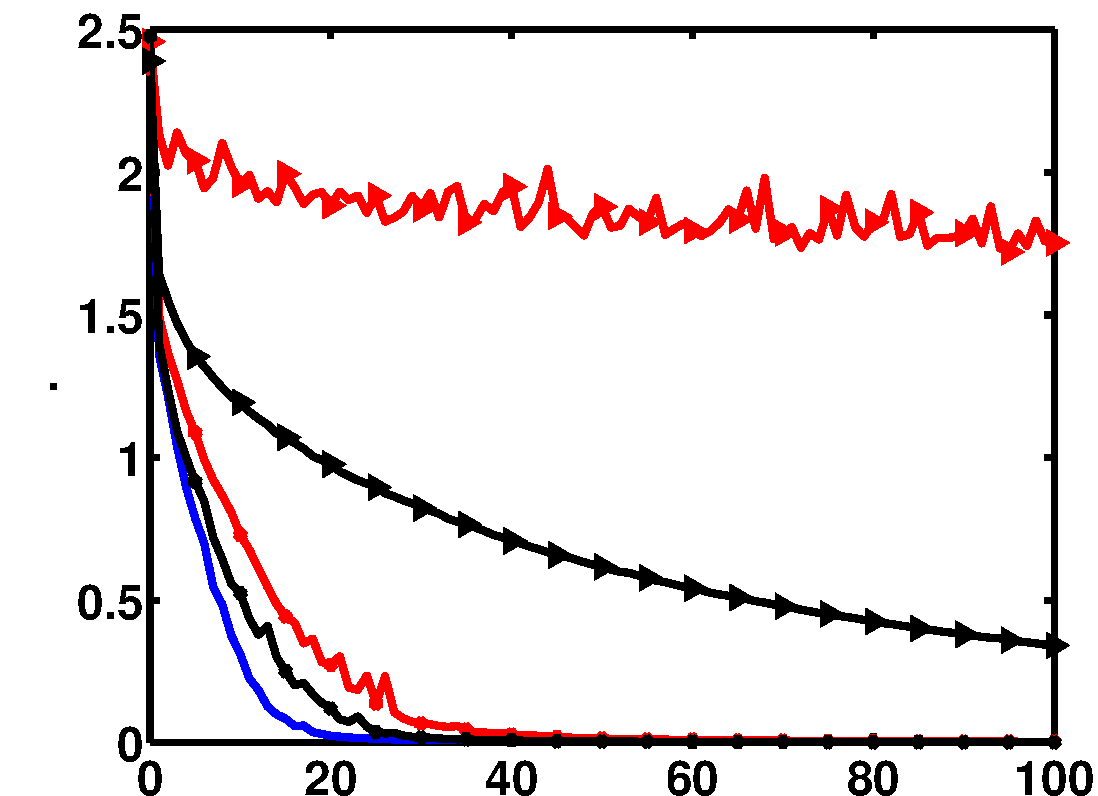
\includegraphics[scale=0.16]{cifar10-surr.pdf} & 
		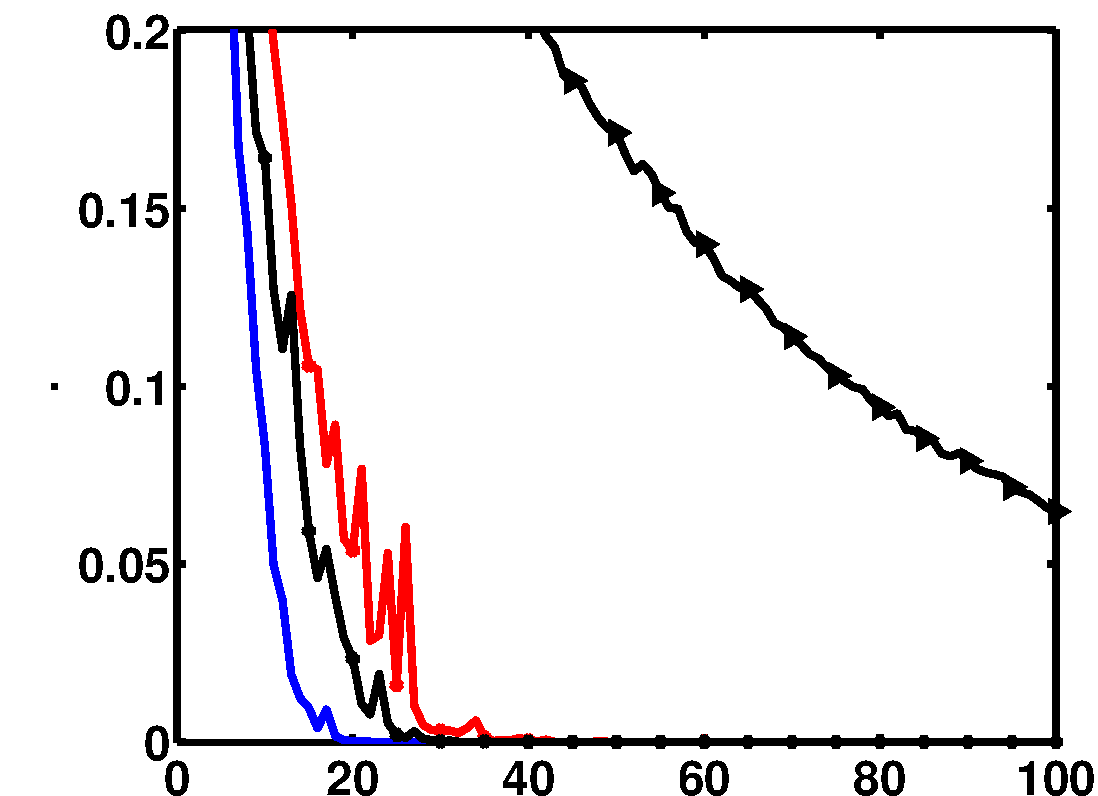
\includegraphics[scale=0.16]{cifar10-train.pdf} &
		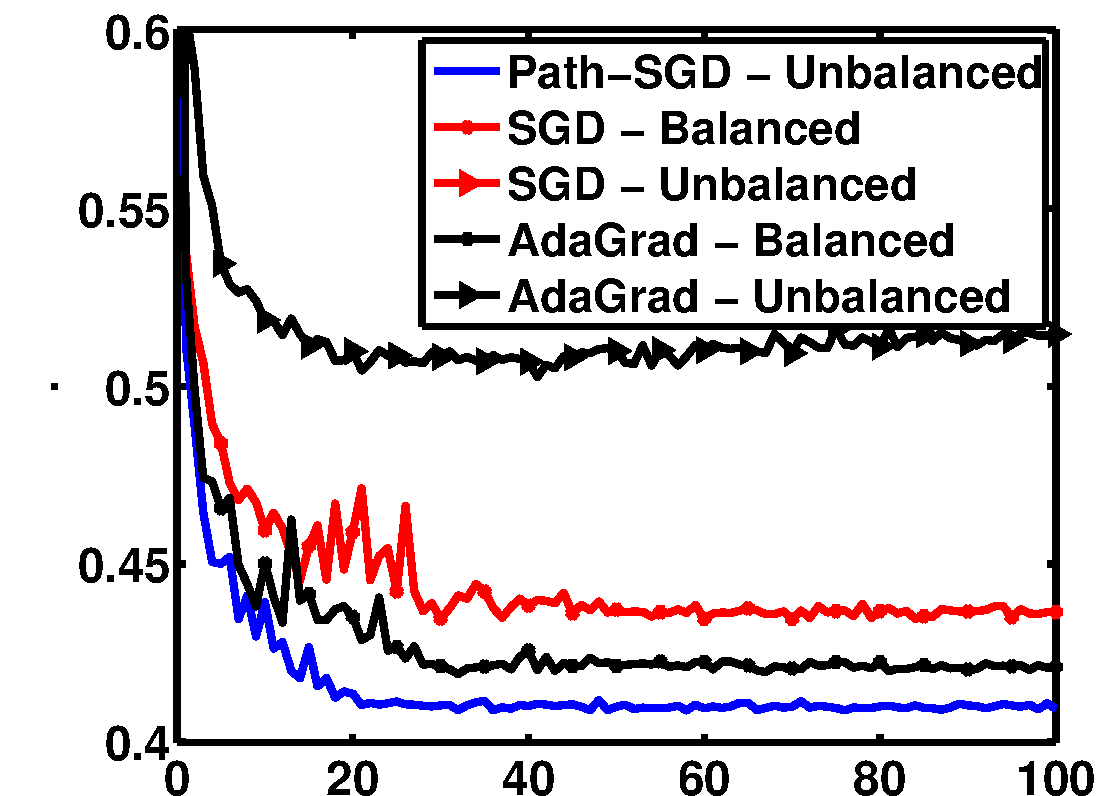
\includegraphics[scale=0.16]{cifar10-test.pdf} 
	\end{tabular} 
	\begin{picture}(0,0)(0,0)
	\rotatebox{90}{\put(342, 0){CIFAR-10}}
	\end{picture}
	\begin{picture}(0,0)(0,0)
	{\put(30, 420){\small Cross-Entropy Training Loss}\put(187, 420){\small 0/1 Training Error}\put(328, 420){ \small 0/1 Test Error}}
	\end{picture}
	\caption{\small to be filled}
	\label{fig:nodrop}
	\vspace{-0.1in}
\end{figure}
\end{frame}
\section{Conclusion}

\end{document}